\documentclass{article}
\usepackage[utf8]{inputenc}
\usepackage[margin = 0.8in]{geometry}
\usepackage{graphicx}
\usepackage{amsmath, amssymb}
\usepackage{subcaption}
\usepackage{multirow}
\usepackage{mathtools}
\usepackage{float}


\title{CS534 - HW 1}
\author{Keith Chester}
\date{Due date: June 12 2022}

\begin{document}
\maketitle

\section*{Problem 1}

In this problem, we were tasked with exploring the \textbf{ReflexVacuumAgent} and a rules based agent, the \textbf{RuleVacuumAgent}. The code for this problem can be found in the attached file of $problem1.py$.

\section*{Problem 2}
Suppose that two friends live in different cities within the map provided from our textbook Figure 3.1, presented below.

\begin{figure}[H]
    \centering
    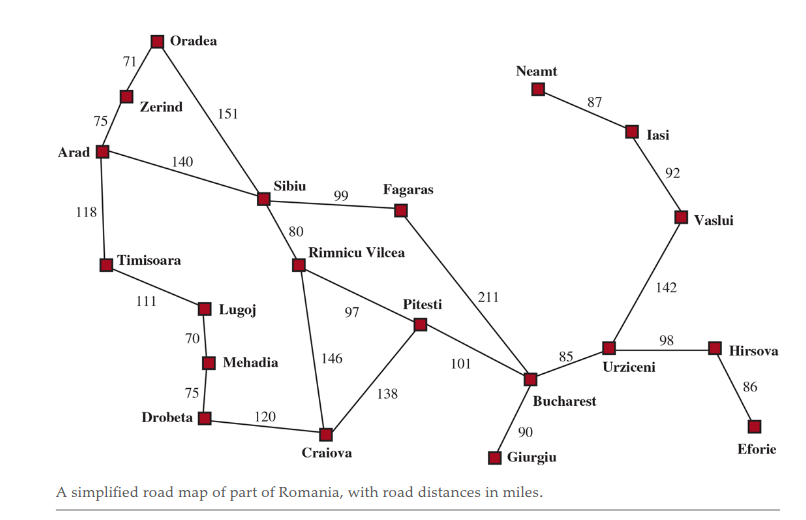
\includegraphics[width = 0.65\textwidth]{imgs/figure31.png}
    \label{fig:fig31}
\end{figure}

The amount of time needed to move from city $i$ to neighbor $j$ is equal to the road distance $D(i,j)$ between the cities. On each turn the friend that arrives first must wait until the other arrives before the next turn of travel can begin. Thus we are limited to the travel time of the slowest agent. We aim to get these friends to meet as quickly as possible.

\subsection*{1. Detailed Problem Formulation}
For our problem, we have two friends - $f_1$ and $f_2$. We wish to find a path such that both end up in the same city $c_{goal}$, at the same time, in the lowest possible time $t$. We have a cost between cities, a distance defined by $D(i,j)$ where $i$ and $j$ are adjacent cities. A given state is defined as $c_{f_1}$ and $c_{f_2}$, which is the city for each given friend. A given action on each discrete step is each friend moving to a new $c_{f_{1/2}}$ until they equal eachother.

\subsection*{2.Which heuristic functions are admissible?}
Suppose that $D(i, j)$ is the straight line distance between cities $i$ and $j$. Which of the following heuristic functions are admissibile?

\begin{itemize}
    \item $D(i,j)$
    \item $2D(i,j)$
    \item $\frac{D(i,j)}{2}$
\end{itemize}

\noindent To be admissible, the heuristic must not overestimate the actual cost of a given transition. Thus the second option, $2D(i,j)$, would not be admissible. The first and third options, $D(i,j)$ and $\frac{D(i,j)}{2}$, respectively, would be admissible.

\subsection*{3. Can a completely connected map have no solutions?}
Yes - since both travelers must travel at the same time, it's possible that a fully connected graph, such as a simple two node map. As both leave for the other's city, they find themselves in opposite cities again. This repeats forever.

\subsection*{4. Are there maps which every solution would require revisting a city?}
Yes. Consider a map with a singular path, with a cycle on the far end, to the side of the second friend's starting position. For example:

\begin{figure}[H]
    \centering
    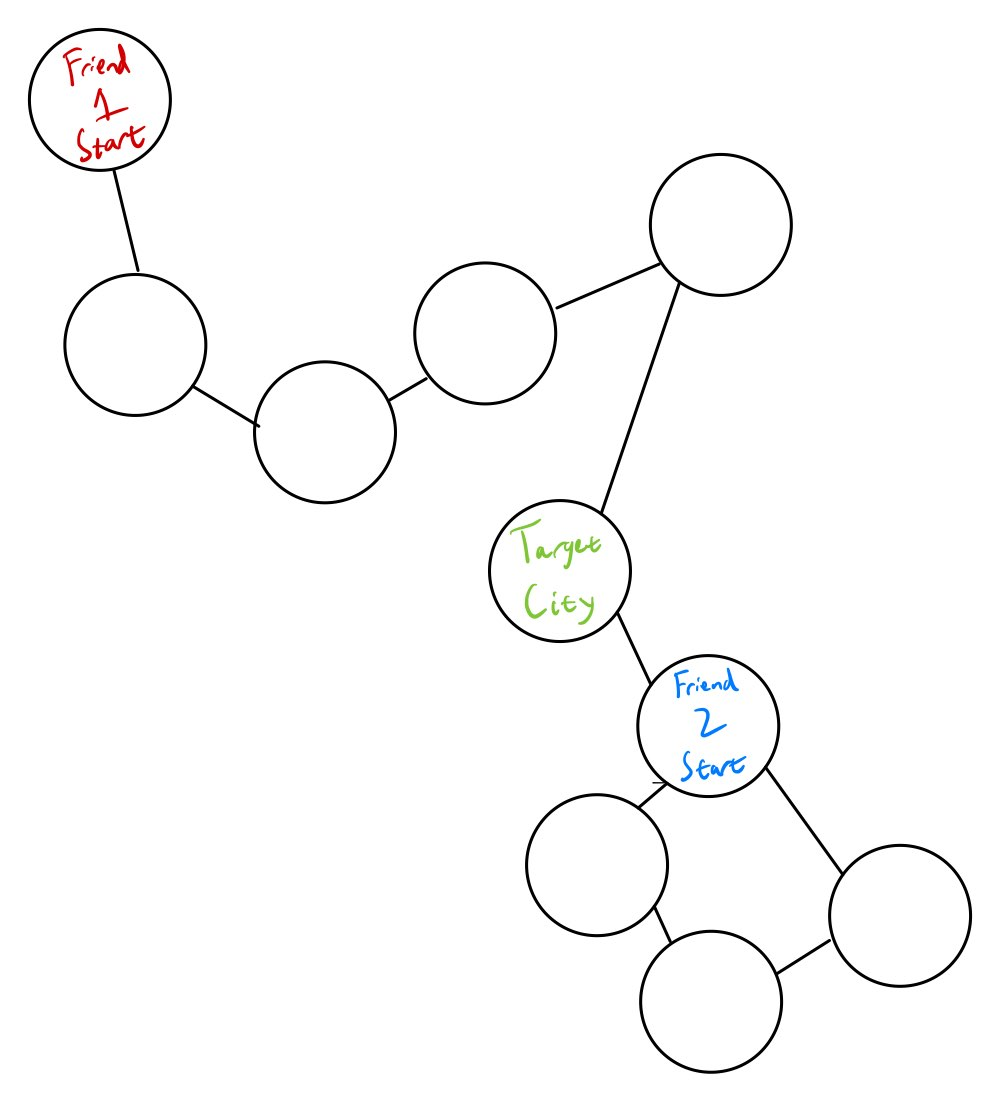
\includegraphics[width = 0.65\textwidth]{imgs/grid_example.jpg}
\end{figure}

\section*{Problem 3}

In this problem we explore a simple hill climbing agent and a genetic algorithm client.

\subsection*{Part A and B}

In this section, we built the traveling salesman problem via the code provided, and then created a genetic algorithm agent to solve the problem as well. The code for this can be found in the paired file $problem3.py$.

\subsection*{Part C}

Here we compare the performance and utilization of the hill climbing agent and the genetic algorithm agent we built.

\begin{center}
    \begin{tabular}{ l r r }
         Agent &     Time to solution &    Fitness of solution \\ 
        Hill Climbing & 6.19 seconds &        1589.8 meters \\  
        Genetic Algorithm & 35.29 seconds  &      2265.6 meters  \\
        Genetic Algoirthm w/ Early Termination & 0.4 seconds & 3132.8 meters \\
    \end{tabular}
\end{center}

We see here that hill climbing quickly finds a solution within 6 seconds, and routinely finds $1589.8$ meters as a solution. Often, however, it finds a close but not as low a value, as it ges stuck on a local minimum.

The genetic algorithm takes far long - 30+ seconds routinely - and in many runs never found a solution that was as low as the hill climbing solution. Since we carry over the top $5$ performers to the next generaton, we have the option of detecting if the top performer has not changed within a number of generations - a form of early termination. When we enable this, the egenetic algorithm quickly finds an answer - usually over 3000 meters, however.

It seems that hill climbing algorithm outperforms genetic algorithms for this problem.

\section*{Problem 4}

In this problem, we are asked to summarize how the minimax algorithm and alpha-beta pruning change their behaviour when we are playing non-zero-sum two player games with separate but known utility functions for each player.

First, we shall expand on some terms to establish a baseline for the discussion. By non-zero-sum we mean that there exists game states in which both of the agents can win - a victory for one does not necessarily mean a defeat for the other. By a utility function, we mean an act of evaluating the state to calculate a score of a given action.

Assume that we have our current player, $A$, and our subsequent opponent, $B$, playing and we wish to calculate the best move for $A$ using minimax. 

Since there is no "minimum" - as both agents can win - we end up not worrying about what the agent $A$, and usually result in a "max-max" instead of a "max-min" result.

\subsection*{Part A}

While minimax still works for our agent, alpha-beta pruning will not work in this situation. Typically, alpha-beta pruning would remove branches where a move by agent $A$ can be forced into a poor position by agent $B$. Since we're in a non-zero-sum situation, these situations are detached and there does not exist a situation where $A$ can be forced by $B$ into a worse position. Therefore we have no significant signals from which we can determine to prune branches of potential actions.

\subsection*{Part B}

If the player's utility functions for a given state can only differ by at most a constant $k$, making the game nearly cooperative, will minimax work? Will alpha-beta pruning?

Minimax still works, but it will operate similarly to before - at both stages the max value will be chosen for each potential agent, or a "maximax" algorithm. As a result alpha-beta pruning will not have the ability to force a particularly bad outcome for $B$, and there will be no real way to determine what branches to prune.

\subsection*{Part C}
If the player's utility functions on any state sum to a number between $-k$ and $k$, making the game essentially zero-sum, we would be in a different situation entirely. We would begin to see moves by $B$ that could directly hurt $A$'s standing - therefore we now have use of the alpha-beta pruning to begin eliminating branches that allow $B$ to force $A$ down a worse path.

\section*{Problem 5}

In this problem we are considering placing $k$ knights on an $nxn$ chessboard such that no two knights are attacking one another, where $k$ is given and $k \leq n^2$.

In this section we aim to choose a $CSP$ formulation. What would the variables be for this problem?


\subsection*{Part A - Variables}

To that end, I submit that we would combine the coordinates of each knight of the $k$ knights into a singular set.

\subsection*{Part B - Possible Values}

The possible values of the variables - also known as the domain of the problem - is a list of all vectors within the set $ \lbrack n^2 \rbrack$. These vectors are expressions of coordinates for the given chess board - $(x,y)$.

\subsection*{Part C - What are your constraints?}

For this problem, our constraints are as follows. We must first limit the placement of the knights such that they aren't in the same square.

Continuing with this, there exists an offset for each given knight, some change of $(\Delta x_{k_a}, \Delta y_{k_a})$ exists that represents the set of all moves from a given $k_a$'s position of $(x,y)_{k_a}$. This set can be up to 8 moves large, depending on the position of the knight (knights placed near edges or corners will have less available legal moves). We must ensure that this given moveset does not result in an equivalent position of a given $(x,y)_{k_b}$.

\begin{itemize}
    \item $(x,y)_{k_a} \neq (x,y)_{k_b}$ - Knights may not exist in the same space
    \item $(\Delta x_{k_a}, \Delta y_{k_a}) \neq (x,y)_{k_b}$ - the potential landing spots for each knight must not be equal to the position of another knight
\end{itemize}

\end{document}